\documentclass[15pt,twoside]{report}
\usepackage[utf8]{inputenc}


\usepackage[a4paper,width=150mm,top=25mm,bottom=25mm,bindingoffset=6mm]{geometry}
\usepackage[british]{babel}
\usepackage{csquotes}

\usepackage{graphicx}
\usepackage{float}
\usepackage{fancyhdr}
\usepackage[nohyperlinks, printonlyused, withpage, smaller]{acronym}
\usepackage[backend=biber, sorting=nyt, style=ext-authoryear-comp,dashed=false,block=par]{biblatex}
\usepackage[inkscapeformat=png]{svg}
\usepackage{booktabs,multirow,array}
\usepackage{listings}
\usepackage{xcolor}
\usepackage{amsmath}

\usepackage[font=small,labelfont=bf,tableposition=top]{caption}
\usepackage{tikz}
\usepackage{tocloft}
\usepackage{enumitem}
\usepackage{appendix}
\usepackage{mathrsfs}
\usepackage{subcaption} % For subfigures
\usepackage{pgfplots}
\usepackage{ragged2e}
% \title{\Large \textbf{Application of Natural Language Processing \\ and Machine Learning in E-Commerce} \\ \Large Predicting Product Taxonomy}
\usetikzlibrary{shapes,arrows,positioning,arrows.meta,calc}
\captionsetup[table]{skip=5pt}

% Customize list of figures appearance in table of contents
\renewcommand{\cftfigpresnum}{\figurename\ }
\setlength{\cftfigindent}{0pt}
\setlength{\cftfignumwidth}{6.5em}

% Add extra space between paragraphs
\setlength{\parskip}{10pt} % Adjust the value to your preferred paragraph spacing



\definecolor{codegreen}{rgb}{0,0.6,0}
\definecolor{codegray}{rgb}{0.5,0.5,0.5}
\definecolor{codepurple}{rgb}{0.58,0,0.82}
\definecolor{backcolour}{rgb}{0.95,0.95,0.92}




% Define the page style "mystyle" for the fancyhdr package
\fancypagestyle{mypagestyle}{
     % Clear all header and footer fields
     \fancyhf{}
     % Set the header to display the chapter name on the right side
     \fancyhead[R]{\leftmark}
     % Set the footer to display the page number on the center
     \fancyfoot[C]{\thepage}
     % Set the footer line to appear (change 0pt to desired line thickness)
     \renewcommand{\footrulewidth}{0.4pt}

}

\lstdefinestyle{mystyle}{
    backgroundcolor=\color{backcolour},   
    commentstyle=\color{codegreen},
    keywordstyle=\color{magenta},
    numberstyle=\tiny\color{codegray},
    stringstyle=\color{codepurple},
    basicstyle=\ttfamily\footnotesize,
    breakatwhitespace=false,         
    breaklines=true,                 
    captionpos=b,                    
    keepspaces=true,                 
    numbers=left,                    
    numbersep=5pt,                  
    showspaces=false,                
    showstringspaces=false,
    showtabs=false,                  
    tabsize=2
}

\lstset{style=mystyle}

\graphicspath{ {images/} }

% \renewbibmacro*{url+urldate}{%
%   \printfield{url}%
%   \iffieldundef{urlyear}
%     {}
%     {\setunit*{\addspace}%
%      \printtext[urldate]{\printurldate}}}

\DeclareFieldFormat{url}{Available at\addcolon\space\url{#1}}
\DeclareFieldFormat{urldate}{\newline Accessed on\addcolon\space{#1}}
% \DeclareFieldFormat{title}{\newline{#1}}
\DeclareFieldFormat{biblabeldate}{#1}
\DeclareDelimFormat{nameyeardelim}{\addcomma\space}% comma before the year
% \DeclareFieldFormat{url}{\bibstring{urlfrom}\addcolon\space\url{#1}}
% \DeclareFieldFormat{urldate}{\mkbibbrackets{\bibstring{urlseen}\addcolon\space#1}}

% \renewbibmacro*{url+urldate}{% changes the default order of the fields url and urldate
%                              \usebibmacro{urldate}%
%                              \newunit
%                              \usebibmacro{url}%
%                             }

%                             \makeatletter
%                             \setlength{\bibitemsep}{0.5\baselineskip plus 0.5\baselineskip}
                            
%                             \newsavebox\ay@labelbox
%                             \newlength{\labwidthsameline}
%                             \setlength{\labwidthsameline}{6em}
                            
%                             % \newbibmacro{labelwidthbib}{%
%                             %   \begingroup
%                             %   \delimcontext{parencite}%
%                             %   \DeclareFieldFormat{bibhyperref}{##1}%
%                             %   \csuse{blx@hook@cite}%
%                             %   \csuse{blx@hook@citekey}%
%                             %   \global\undef\cbx@lasthash
%                             %   \global\undef\cbx@lastyear
%                             %   \citetrackerfalse\pagetrackerfalse\backtrackerfalse
%                             %   \defcounter{maxnames}{\blx@maxcitenames}%
%                             %   \printtext[brackets]{\usebibmacro{cite}}%
%                             %   \endgroup
%                             % } 
%                             %-----------------------
%                             \newbibmacro{kicklabel}{% 
%                               \sbox\ay@labelbox{\usebibmacro{labelwidthbib}}%
%                               \global\togglefalse{blx@insert}%
%                               \ifdim\wd\ay@labelbox>\labwidthsameline
%                                 \leavevmode\newline
%                               \fi
%                             }
                            
%                             \defbibenvironment{bibliography}%
%                               {\list
%                                 {\usebibmacro{labelwidthbib}}%
%                                 {\setlength{\labelwidth}{\labwidthsameline}%
%                                  \setlength{\leftmargin}{\labelwidth}%
%                                  \setlength{\labelsep}{\biblabelsep}%
%                                  \addtolength{\leftmargin}{\labelsep}%
%                                  \setlength{\itemsep}{\bibitemsep}%
%                                  \setlength{\parsep}{\bibparsep}%
%                                  \renewcommand*{\makelabel}[1]{##1\hss}}}%
%                               {\endlist}%
%                               {\item\usebibmacro{kicklabel}}
%                             \makeatother

\addbibresource{References.bib}

\includeonly{preliminary/title, %
preliminary/affidavit, %
preliminary/certificate, %
preliminary/acknowledgement, %
preliminary/abstract, %
preliminary/acronyms, %
chapters/introduction, %
chapters/literature, %
chapters/methodology, %
chapters/experiment, %
}

\begin{document}


%--------------- Prelimanary pages -------------


%--------------------------------------------
\begin{titlepage}

    \vspace*{3\baselineskip}
        \begin{flushright}        
  
                
\includegraphics[scale=0.3]{SRH_Hochschule_Heidelberg_logo.svg.png}
           
        \end{flushright}
    \vspace*{3\baselineskip}

    \centering
   


    {\Large \bfseries Application of Natural language processing in E-Commerce \\ Predicting product taxonomy}
    \vspace*{3\baselineskip}

    {\Large Master Thesis}
    \vspace*{1\baselineskip}

    {\Large by }
    \vspace*{2\baselineskip}

    {\Large  \bfseries Shoney Arickathil }
    \vspace*{0.5\baselineskip}

    {\Large  Student no: 11017678 }
    \vspace*{2\baselineskip}

    {\Large \today}
    \vspace*{8\baselineskip}

    % \includegraphics[width=0.35\linewidth]{srhlogo}

    {\Large  Masters in Applied Computer Science }
    \vspace*{0.5\baselineskip}

    {\Large  SRH University Heidelberg \\ School of Informatics}  
    \vspace*{6\baselineskip}

    \begin{minipage}{\textwidth}
        \begin{flushleft} % Left-align supervisor's name
            \large Primary Supervisor: \hfill \bfseries Prof. Dr. Gerd Moeckel
           
        \end{flushleft}
       
       
    \end{minipage}

    


   
    
\end{titlepage}

\begin{titlepage}
    \begin{flushright}
        
  
\section*{Declaration}
\justifying {
I hereby declare that the work presented in this Project Report titled \textbf{ Machine Learning for traffic flow prediction at different junctions – M.Tech}. Submitted to the \textbf{ Indian Institute of Technology Jodhpur} in partial fulfilment of the requirements for the award of the degree of M.Tech (Masters of Technology), is a Bonafide record of the research work carried out under the supervision of \textbf{ Dr. Ranju Mohan}. The contents of this Project Report in full or in parts, have not been submitted to, and will not be submitted by me to, any other Institute or University in India or abroad for the award of any degree or diploma.
}
\vspace*{3\baselineskip}


{\large \bfseries Cyril John Arickathil \par}
{\large \bfseries M22RM210 \par}


\end{flushright}

\end{titlepage}


\begin{titlepage}
    \begin{flushright}
        
  
\section*{Certificate}
\justifying
This is to certify that the Project Report titled \textbf{Machine Learning for traffic flow prediction at different junctions}, submitted by \textbf{Cyril John Arickathil (M22RM210)} to the \textbf{Indian Institute of Technology Jodhpur} only for the award of the degree of \textbf{M.Tech in Robotics and Mobility Systems (RMS)} is a Bonafide record of the work under my supervision. To the best of my knowledge, the contents of this report, in full or in parts, have not been submitted to any other Institute or University for the award of any degree or diploma.
\vspace*{3\baselineskip}




{\large  \bfseries  Dr. Ranju Mohan }


\end{flushright}

\end{titlepage}


\begin{titlepage}
    \begin{flushright}
        
  
\section*{Acknowledgment}
\justifying
I would like to extend my deepest gratitude to \textbf{ Dr. Ranju Mohan} for her invaluable guidance
and support as my project supervisor. Her insightful feedback, unwavering encouragement, and
extensive knowledge have been instrumental in the successful completion of this project. Dr.
Mohan's dedication to excellence and her willingness to share her expertise have greatly
enhanced my learning experience. I am truly grateful for her mentorship and the opportunity
to work under her supervision. Her insights and expertise were crucial to the successful
completion of this work.

I am also immensely grateful to my examiners, \textbf{Dr. Bhupendra Singh} and Dr. Riby Abraham
Boby, for their thorough evaluation, constructive feedback, and suggestions, which greatly
contributed to the enhancement of this project.

My heartfelt thanks go to the program coordinators, \textbf{ Dr. Gourav Bhatnagar} and Dr. Dilpreet
Kaur, for their unwavering support, efficient coordination, and assistance in all administrative
matters, making this academic journey a smooth and enriching experience.
Finally, I would like to acknowledge the support and encouragement from my family,my elder brother, friends,
and colleagues, without whom this project would not have been possible.
\vspace*{3\baselineskip}


Thank you, \\

{\large  \bfseries Cyril John Arickathil }


\end{flushright}

\end{titlepage}

\begin{abstract}
    

\begin{center}
    Shoney Arickathil, School of Informatics, SRH Hochschule Heidelberg \\

Master Thesis \\
\textbf{Application of Natural language processing in ECommerce}\\
\textbf{Predicting product taxonomy}

\end{center}


Electronic commerce started in early 1990's in which the business transactions are conducted through computer networks. The ease of buying a product online has reduced physical work and time required for decision-making by compare the product features. A wide range of products are sold online. One of the challenge is to well define a products' taxonomy. A product taxonomy is a hierarchical structure to organize the products in an E-commerce platform in such a way that customers can find the product in the fewest possible clicks.
Product taxonomy for the same product may differ based on the supplier and manufacturer (sources). Hence, product taxonomy details cannot be imported directly from the sources into the E-commerce platform. Product details cannot be live until its taxonomy is not well-defined, this delays the time of product availability for customers. 

In this thesis the author developed a machine learning classification model to predict the product taxonomy based on the features of the product. This is achieved with machine learning model. Experimenting and analyzing by varying  model's parameters facilitated to determine models performance.  

Initially, from the existing product taxonomy the features such as name and description were extracted. These extracted features were passed through process of text normalization, imputation of missing text to standardize it before converting it into One-Hot encoded format. These features and its lowest hierarchical level of category were processed by \acf*{RNN} machine learning model to learn the patterns of feature and classify it with the concept of probability distribution.

The result of predicting the lowest hierarchical level of product category based only on product name formed a foundation to create a machine learning model to predict the complete product taxonomy. As the level of category to be predicted increases the model's weight and product features need to be adjusted. 

\end{abstract}





\pagenumbering{roman}
\pagestyle{plain}
\tableofcontents

\clearpage
%----------------- chapters --------------------
\pagestyle{mypagestyle}
\pagenumbering{arabic}

%---------------------------------------
\chapter{Introduction}

\section{Topic overview}


\chapter{Literature survey}

\section{Supervised Learning}

The machine learning model built using existing dataset is called supervised learning. ´Figure1 illustrates the supervised learning workflow. In this paper, author builds a supervised learning model to predict the product taxonomies. The work flow starts with data collection, this step involves fetching the corpus of raw data. This raw data processed before creating a training data set out of it. The data preprocessing steps involves feature selection, text normalization, data imputation and feature extraction. The training data is passed an input to the model which compares its results with the actual value to self- evaluate and learn. If any hyperparameter tuning for the machine learning model is required then it is trained again with new parameters. The model is then evaluated and then deployed for production use.
\begin{figure}[h!]
    \centering    
    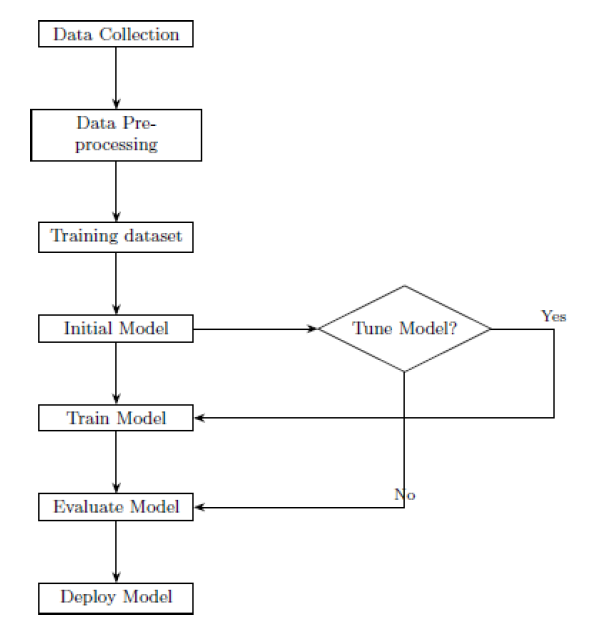
\includegraphics[scale=0.8]{supervised_learning.png}
    \caption{Supervised Learning}
\end{figure}


\section{Machine Learning Techniques in Traffic Prediction}

Machine learning techniques have shown great promise in traffic flow prediction due to their ability to learn from data and capture complex patterns. Key machine learning techniques explored in the literature include:

\begin{itemize}
    \item Linear Regression
    \item Decision Trees and Random Forest
    \item Support Vector Machines (SVM)
    \item Neural Networks
    \item Deep Learning Models (Recurrent Neural Networks (RNN), Long Short-Term Memory (LSTM))
 
    

\end{itemize}

\section{Comparative Studies}

Several comparative studies have evaluated the performance of different machine learning models in traffic flow prediction. These studies provide insights into the strengths and weaknesses of various models, guiding the selection of appropriate techniques for specific scenarios.




\chapter{Methodology}

\section{Start with small prototype}

Predicting the number of vehicles on a particular junction involves processing timeseries data. Initially the author processes the data only forone of the junction. The raw data has been used from Kaggle.com provided by  \parencite{fedesoriano}.

About the dataset : \\
The dataset contains data from year 2015-2017 along with junctions and number of vehicles in hourly intervals.
The data manipulation is performed using Python library-Pandas.

\begin{lstlisting}[language=Python,caption={Data set fetching using Pandas},label={code:data}]
    df = pd.read_csv('Data/traffic.csv')
    df = df.drop('ID', axis=1) df.head()
\end{lstlisting}

\begin{lstlisting}[language=Bash,caption={Sample Result},label={code:confusion matrix}]
    index,DateTime,Junction,Vehicles,ID
    0,2015-11-01 00:00:00,1,15,20151101001
    1,2015-11-01 01:00:00,1,13,20151101011
    2,2015-11-01 02:00:00,1,10,20151101021
    3,2015-11-01 03:00:00,1,7,20151101031
    4,2015-11-01 04:00:00,1,9,20151101041
\end{lstlisting}

At 4 junctions vehicles passing in every 1 hour recorded. Entire test dataset available in  ``traffic.csv'' file

\section{Time series extraction}

Developing a machine learning model to predict the flow of traffic considering multiple aspects such as exact point of year(month-wise), also on the daily basis considering progression hour-wise is a complicated process.

We need to split the data such that \texttt{DateTime} column is split into `months', `hours', `day'. This is important as various aspects such as `day of the week', `month in a year', `hours in a day' need to be checked against for validating the trend in traffic.

\begin{lstlisting}[language=Python,caption={Data set fetching using Pandas},label={code:data}]
    df['DateTime'] = pd.to_datetime(df['DateTime'], format='mixed')
    # Exploring more features
    df_Junction1["Year"]= df_Junction1['DateTime'].dt.year 
    df_Junction1["Month"]= df_Junction1['DateTime'].dt.month
     df_Junction1["Date_no"]= df_Junction1['DateTime'].dt.day 
     df_Junction1["Hour"]= df_Junction1['DateTime'].dt.hour 
     df_Junction1["Day"]= df_Junction1.DateTime.dt.strftime
     ("%A") df_Junction1.head()
\end{lstlisting}




\section{Ideate: Data Exploration}

Initial approach of finding a solution to predict time-series event is to analyze already existing solution to a different type of prediction problem.

For example, \parencite[Section 4.3]{Goodfellow-et-al-2016} showcases the implementation of RNN (Recurrent Neural Network) techniques in handling time-series events. In this context, the author leverages historical data patterns, to forecast the progression of traffic over time. The primary goal is to predict traffic conditions based on learned historical patterns.

In tailoring this methodology to the intricacies of traffic flow, the author recognizes the complexity of the task and opts to utilize past data patterns for making predictions.

To assess the effectiveness of the model, the author employs a visual tool, such as plotting graphs based on various traffic events. This visual representation offers a clear evaluation of predicted versus actual traffic conditions. Additionally, this approach allows for manual verification and scrutiny of instances where the model may have inaccurately predicted traffic conditions, contributing to a more comprehensive understanding of the model's performance.


\section{Understanding Mathematics of Neural Networks}

In this paper, author researches on the relevance of the mathematical concept with respect to the machine learning process. Understanding the math behind reducing the loss for prediction enables to completely understand the algorithms. Especially the training algorithm applies the activation functions. Author describes the theoretical knowledge with reasoning to apply these activation functions.

Understanding the mathematical foundations on which the neural networks and data prediction model works enables to reverse engineer the algorithm of machine learning model.




\chapter{Experiments and Results}

\section{Experimental Setup}

The experimental setup includes the selection of appropriate datasets, splitting the data into training
and testing sets, and tuning hyperparameters for each model.


\begin{lstlisting}[language=Python,caption={Data set fetching using Pandas},label={code:data}]
    J1 = df[df['Junction']==1]
    J2 = df[df['Junction']==2]
    J3 = df[df['Junction']==3]
    J4 = df[df['Junction']==4]
    vehciles_at_J1 = J1['Vehicles']
    vehciles_at_J2 = J2['Vehicles']
    vehciles_at_J3 = J3['Vehicles']
    vehciles_at_J3 = J3['Vehicles']
\end{lstlisting}

\begin{lstlisting}[language=Bash,caption={Sample Result},label={code:confusion matrix}]
    #save
    #logic take input for first 5 hours and
    # predict 6th hour
    # [[1],[2],[3],[4],[5]] [6]
    # [[2],[3],[4],[5],[6]] [7]
    # [[3],[4],[5],[6],[7]] [8]
    def df_to_X_y(df, window_size=5):
    df_as_np = df.to_numpy()
    X =[]
    y = []
    for i in range(len(df_as_np)-window_size):
    row = [[a] for a in
    X.append(row)
    label = df_as_np[i+window_size]
    y.append(label)
    return np.array(X), np.array(y)
\end{lstlisting}

\clearpage

\section{Performance Metrics}

Performance metrics used to evaluate the models include Mean Absolute Error (MAE), Mean Squared Error (MSE), and R-squared (R\textsuperscript{2}).


\begin{lstlisting}[language=Python,caption={Performance Metrics},label={code:data}]
    model1 = Sequential()
    model1.add(LSTM(64, input_shape=(WINDOW_SIZE, 1)))
    model1.add(Dense(8, 'relu'))
    model1.add(Dense(1))
    model1.compile(loss=MeanSquaredError(), optimizer=Adam(learning_rate=0.001), metrics=[RootMeanSquaredError()])
    model1.summary()
\end{lstlisting}




\section{Results and Analysis}

The results of the experiments are analyzed to compare the performance of different models and identify the most effective approaches for traffic flow prediction.

\begin{lstlisting}[language=Python,caption={Performance Metrics},label={code:data}]
    from tensorflow.keras.models import load_model
    model1 = load_model('model1/')
    train_results['Train Predictions'][:150].plot()
    train_results['Train Actual'][:150].plot()
\end{lstlisting}



\begin{figure}[h!]
    \centering
    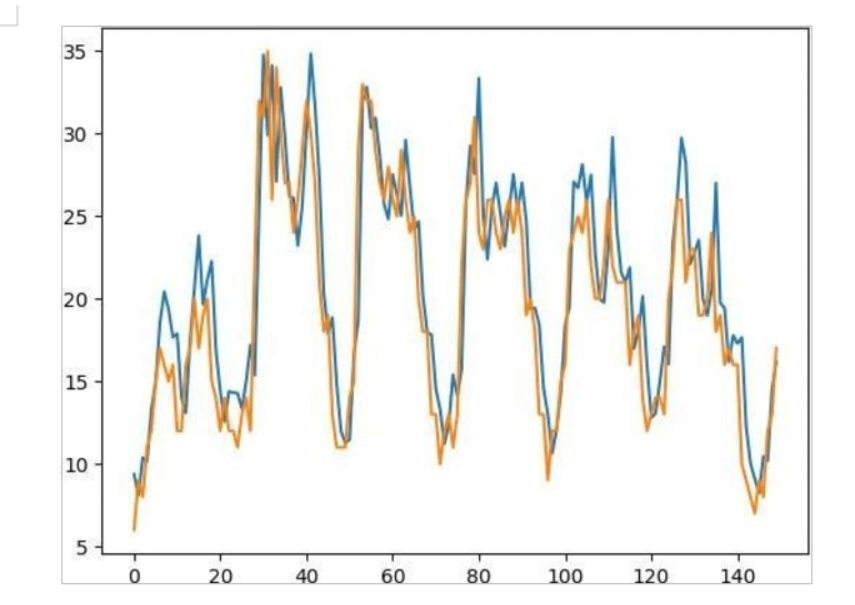
\includegraphics[width=\textwidth]{result2.png}
\end{figure}


\begin{lstlisting}[language=Python,caption={Performance Metrics},label={code:data}]
    val_predictions = model1.predict(X_val).flatten()
    val_results = pd.DataFrame(data={'Validation Predictions':val_predictions, 'Validation Actual':y_val})
    val_results
    val_results['Validation Predictions'][:150].plot()
    val_results['Validation Actual'][:150].plot()
\end{lstlisting}

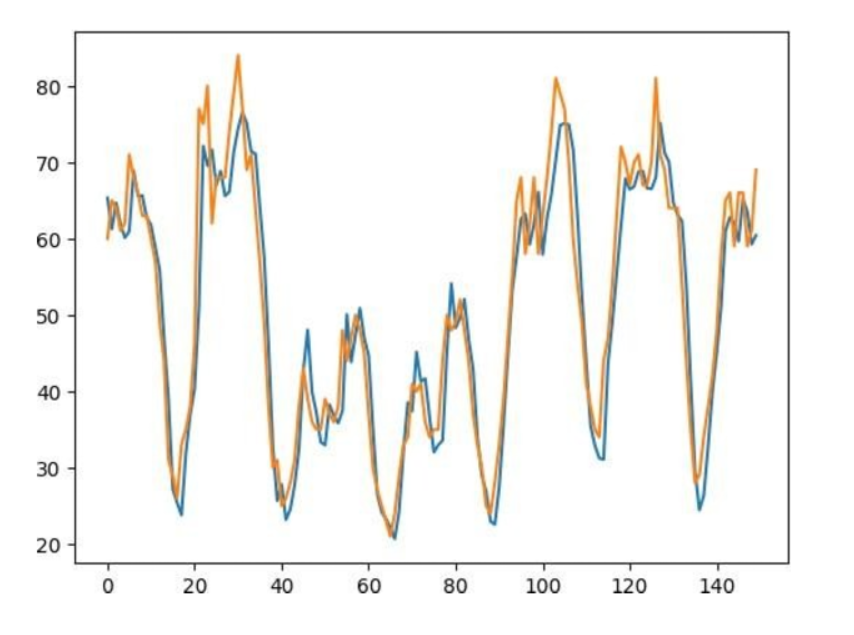
\includegraphics[scale=1]{result_1.png}

\pagenumbering{roman}
\pagestyle{mypagestyle}

% Add the List of Figures to the table of contents
\cleardoublepage % Ensure the correct page
\addcontentsline{toc}{chapter}{\listfigurename}
\listoffigures


\addcontentsline{toc}{chapter}{\listtablename}
\listoftables

\lstlistoflistings


\clearpage
% \printglossary[type=\acronymtype]

% \printglossary
\addcontentsline{toc}{chapter}{Bibliography}


\nocite{*}
\printbibliography[title={References}]



% \defbibheading{bibempty}{}

% \let\oldbib\thebibliography
% \let\endoldbib\endthebibliography
% \renewenvironment{thebibliography}
%   {\vspace{\baselineskip}\begin{oldbib}}
%   {\end{oldbib}\vspace{\baselineskip}}


\end{document}